\documentclass[10pt]{article}
\usepackage[margin=2cm, a5paper]{geometry}

\usepackage{amsmath, amsthm, amssymb}

\usepackage[dvipsnames]{xcolor}
\usepackage{tikz}
\usepackage{pgfplots}

\usepackage[hidelinks]{hyperref}

% \usepackage[skip=0.15cm]{parskip}

\usepackage{subcaption}
\usepackage{graphicx}

\usepackage{verbatim}

\usepackage{libertinust1math}
\usepackage{libertine}

\usepackage{inconsolata}

\DeclareCaptionLabelSeparator{custom}{.}
\DeclareCaptionFormat{custom}{\textbf{#1#2} #3}

\captionsetup{
  format=custom,
  labelsep=custom
}

\newtheoremstyle{customthm}
{}{}{}{}
{\scshape \bfseries}{.}{ }{}
\theoremstyle{customthm}
% \theoremstyle{definition}
\newtheorem*{definition}{Definition}
\newtheorem*{lemma}{Lemma}

\newenvironment{cproof}[1][\proofname]{%
  \proof[\scshape #1]%
}{\endproof}

\renewcommand{\qedsymbol}{\( \blacksquare \)}

\DeclareMathOperator{\uniform}{\textsf{Uniform}}
\newcommand{\Uniform}[2]{\ensuremath{\uniform \left(#1, #2 \right)}}

\DeclareMathOperator{\LaplaceL}{\mathfrak{L}}
\newcommand{\Laplace}[1]{\ensuremath{\LaplaceL \left\{ #1 \right\} (s)}}
\newcommand{\InvLaplace}[1]{\ensuremath{\LaplaceL^{-1} \left\{ #1 \right\} (t)}}

\DeclareMathOperator{\variance}{\mathrm{Var}}
\newcommand{\Variance}[1]{\ensuremath{\variance \left( #1 \right)}}

% TODO:

\begin{document}

\section*{A Restricted Random Walk}

\vspace{-0.2cm}

\textit{Rushil Surti}

\vspace{0.2cm}

These are the updated notes of the restricted random walk details I sent Lester. I've changed them to follow the progression of the presentation more and updated them with some of the stuff I was missing; hopefully they provide some insight :)

The problem: \textit{A particle centered at the origin chooses uniformly a path of length 1. What is the probability distribution of the displacements?}

\subsection*{Overview}

In total, we know that, given the rotational symmetry of the problem, we really only need to consider a single radial cross section of the disk for our distribution.

\begin{figure}[b]
    \centering
    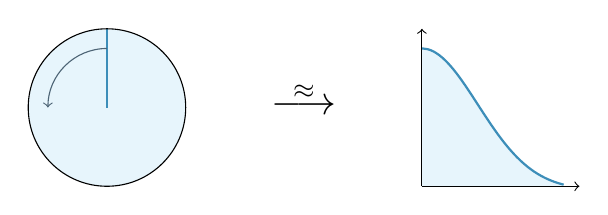
\begin{tikzpicture}
        \fill[Cerulean!10] (-2.5, 0) circle (1);
        \draw[Cerulean!75!black, thick] (-2.5, 0) -- (-2.5, 1);
        \draw (-2.5, 0) circle (1);

        \draw[->, Cerulean!40!black] (-2.5,0.75) arc (90:180:0.75);

        \node (arrow) at (0, 0) {\Large \( \longrightarrow \)};
        \node at (0, 0.2) {\( \approx \)};

        \fill[domain=0:1.8, smooth, thick, Cerulean!10] plot ({\x + 1.5}, {1.8 * exp(-\x * \x) - 1.05}) -- (3.3, -1) -- (1.5, -1) -- cycle;
        
        \draw[domain=0:1.8, smooth, thick, Cerulean!75!black] plot ({\x + 1.5}, {1.8 * exp(-\x * \x) - 1.05});
        
        \draw[->] (1.5, -1) -- (3.5, -1);
        \draw[->] (1.5, -1) -- (1.5, 1);

    \end{tikzpicture}
    \caption{The distribution is rotationally symmetric, so it is completely described by the distribution on a single radial slice.}
\end{figure}

The general solution path we shall take for this is to model a path as a fixed number of steps \( N \) each of length \( 1 / N \) so that the length \( 1 \) condition is satisfied.

Each step is modeled to be a random variable uniformly distributed on a circle of radius \( 1 / N \). Thus, our distribution of paths is the integral, or alternatively infinite summation, of these random variables.

Taking the convolution of these random variables and finding the distribution in two dimensions is difficult, but using the triangle inequality, we can look solely at the \( x \)-component on this circle and see that the \( x \)-component is uniformly distributed on \( [-1/N, 1/N] \).

\subsection*{Mathematical Statement of the Problem}

\begin{definition}
    Let the \textbf{circular distribution} \( \textsf{Circle} (r) \) be uniformly distributed on a circle with radius \( r \), having a probability density function
    \[
        f(x, y) = \frac{1}{2 \pi r} \delta (x^2 + y^2 - r^2)
    ,\]
    where \( \delta(t) \) is the Dirac delta function (we have to use this because otherwise the support of the distribution would have measure \( 0 \), but this is not what causes the Dirac delta distribution in the final answer).
\end{definition}
Suppose we have a continuous stochastic process \( \{ C_r (t) \colon t \in [0, 1] \} \) where each \( C_r (t) \) has a circular distribution. We wish to find the distribution
\[
    \int_0^1 C_{dt} (t) \, dt
.\]

\subsection*{Simplification to Uniform Convolutions}

We can transform the problem to a single dimensional using the aforementioned triangle inequality. Let \( \{ X_r (t) \colon t \in [0, 1] \} \) be a continuous stochastic process where \( X_r (t) \sim \Uniform{-r}{r} \) for all \( t \). We're in particular concerned with the probability density function of the following distribution.
\[
    \int_0^1 X_{dt} (t) \, dt
.\]
To be more clear, this is equivalent to the Riemann sum (at least, assuming this is Riemann integrable)
\[
    \lim_{N \to \infty} \sum_{k = 1}^N X_{(1 / N)} (k / N)
.\]
With this, we are taking the convolution of all the \( x \)-components of possible jumps. Once we have this, we can use the fact that the distribution is rotationally symmetric to extend this to the whole disk distribution\footnote{At least, that's the plan I had in mind, but thinking upon it a bit more, I'm beginning to doubt it. Perhaps I just need to wake my brain up, but I don't think this a transformation that preserves everything completely. Hahahahaha I might be going senile}. In order to actually obtain the probability density function for this, we will have to do a little bit of work.

\begin{lemma}
    The convolution of \( N \) independently, identically distributed random variables \( X_1, X_2, \ldots, X_N \sim \Uniform{-r}{r} \) has the probability density function
    \[
        f(t) = \frac{(2r)^{-N}}{(N - 1)!} \sum_{k = 0}^N \binom{N}{k} (-1)^k (t + (N - 2k)r)^{N - 1} H (t + (N - 2k)r)
    ,\]
    where \( H(t) \) denotes the Heaviside step function.
\end{lemma}

\begin{cproof}
    Take the (bilateral) Laplace transform of probability density function of any of the random variables, \( f_{X_i} (t) \), and denote it by \( U(s) \).
    \begin{align*}
        U(s) := \Laplace{f_{X_i} (t)} &= \int_{-\infty}^{\infty} f_{X_i} (t) e^{-st} \, dt \\
        &= \frac{1}{2r} \int_{-r}^{r} e^{-st} \, dt \\
        &= \frac{1}{2rs} \left( e^{rs} - e^{-rs} \right)
    .\end{align*}
    Using the properties of the Laplace transform, we can convolve the random variables with themselves \( N \) times by taking \( U(s) \) to the \( N \)th power, expanding with binomial theorem.
    \begin{align*}
        \left( U(s) \right)^N &= (2r)^{-N} \sum_{k = 0}^N \binom{N}{k} (-1)^{k} \frac{e^{(n-2k)rs}}{s^N} \\
        \InvLaplace{\left( U(s) \right)^N} &= (2r)^{-N} \sum_{k = 0}^N \binom{N}{k} (-1)^{k} \InvLaplace{\frac{e^{(n-2k)rs}}{s^N}}
    .\end{align*}
    From here we can take the inverse Laplace transform (using a table) to get back our probability density function in terms of \( t \).
    \[
        = \frac{(2r)^{-N}}{(N - 1)!} \sum_{k = 0}^N \binom{N}{k} (-1)^k (t + (N - 2k)r)^{N - 1} H (t + (N - 2k)r)
    .\]
\end{cproof}
This allows us to transform our infinite sum distribution and find its probability density function, which shall be denoted by \( C(t) \). In this case, we take \( r = 1 / N \).
\[
    C(t) := \lim_{N \to \infty} \frac{N^N}{2^N (N - 1)!} \sum_{k = 0}^N \binom{N}{k} (-1)^k (t + (N-2k)/N)^{N - 1} H(t + (N-2k)/N)
.\]
We'll call this distribution of \( x \)-components \( \textsf{Particle} \).

\subsection*{Collapsing to a Dirac Delta}

Motivated by graphing\footnote{\url{https://www.desmos.com/calculator/kuoaqipi0x}}, we can show that the variance of the distribution goes to \( 0 \) as \( N \to \infty \).
\begin{lemma}
    Suppose random variable \( Y \sim \textsf{Particle} \). Then, \( \variance (Y) = 0 \).
\end{lemma}
\begin{cproof}
    Recall that
    \[
        Y = \lim_{N \to \infty} \sum_{k = 1}^N X_k
    ,\]
    where \( X_k \sim \textsf{Uniform} (-1/N, 1/N) \). It follows immediately from the linearity of variance (and that the steps are identically distributed) that
    \[
        \variance(Y) = \lim_{N \to \infty} N \Variance{X_k}
    .\]
    We know that the mean of each \( X_k \) is \( 0 \). This allows us to trivially find the variance of the step \( x \)-components to be
    \begin{align*}
        \Variance{X_k} &= \frac{N}{2} \int_{-1/N}^{1/N} t^2 \, dt \\
        &= \frac{N}{2} \left[ \frac{1}{3N^3} + \frac{1}{3N^3} \right] \\
        &= \frac{1}{3N^2}
    .\end{align*}
    With this, we can find the variance of \( Y \).
    \begin{align*}
        \variance(Y) &= \lim_{N \to \infty} N \cdot \frac{1}{3N^2} \\
        &= 0
    .\end{align*}
\end{cproof}
With this, we can be fairly certain that the particle is almost always at the origin.

\begin{figure}
    \centering
    \begin{tikzpicture}
    \begin{axis}[
        xlabel={Magnitude of displacement},
        ylabel={Frequency},
        axis x line = bottom,
        axis y line = left,
        xmin = 0,
        xmax = 1
    ]
        \addplot[color=Cerulean!75!black, thick] table [x=step, y=frequency, col sep=comma] {empirical.csv};
    \end{axis}
    \end{tikzpicture}
    \caption{The results for a simulation of \( 1000 \) random walks, each taking \( 10000 \) steps.}
    \label{fig:empirical}
\end{figure}

The (likely) last thing one can do to verify results like these is to empirically simulate them. While this specific problem does not lend itself quite well for obtaining an approximate, \textit{continuous} distribution for the positions, we can certainly create a \textit{discrete} one that may give some insight.

In simulating this, we simply generate a large number (\( 1000 \) in this case) of random walks (approximating the Riemann sum with say \( N = 10000 \) steps), take the radius of their ending position, and place them in a graph with bins according to ranges of values. In this case, we take the number of bins to be \( 100 \). This generates the data in Figure \ref{fig:empirical}.

If we increase the number of steps the simulated random walk takes, it gets even closer to simply peaking at \( t = 0 \).

The code for generating Figure \ref{fig:empirical} is:
\verbatiminput{empirical.py}
This generates CSV output for use in graphing in \LaTeX.

\end{document}